\documentclass{article}
\usepackage{graphicx}
\usepackage{wrapfig}
\usepackage{filecontents}
\usepackage{siunitx}
\usepackage[table]{xcolor}
\usepackage{float}
\usepackage{hyperref}

\usepackage{color} % balíček pro obarvování textů
\usepackage{xcolor}  % zapne možnost používání barev, mj. pro \definecolor
\usepackage[total={175mm,230mm}, top=23mm, left=20mm, includefoot]{geometry}
\hypersetup{
    colorlinks,
    linkcolor={blue!50!black},
    citecolor={green!50!black},
    urlcolor={blue!80!black}
}
\definecolor{orange}{RGB}{ 251, 114, 032}
\definecolor{fialova}{RGB}{ 255, 000, 255}

\newcommand \obr[1]
{ obr. \ref{#1}}

\newcommand \tab[1]
{ tab. \ref{#1}}


% \usepackage{lmodern}
% \usepackage{amssymb,amsmath}
% \usepackage{ifxetex,ifluatex}
% \usepackage{fixltx2e} % provides \textsubscript
% \ifnum 0\ifxetex 1\fi\ifluatex 1\fi=0 % if pdftex
%   \usepackage[T1]{fontenc}
%   \usepackage[utf8]{inputenc}
% \else % if luatex or xelatex
%   \ifxetex
%     \usepackage{mathspec}
%   \else
%     \usepackage{fontspec}
%   \fi
%   \defaultfontfeatures{Ligatures=TeX,Scale=MatchLowercase}
% \fi

% \usepackage{pgfplots} % http://www.chiark.greenend.org.uk/doc/texlive-doc/latex/pgfplots/pgfplots.pdf
% \usepackage{blindtext}

% \usepackage{subfiles} % Best loaded last in the preamble

% \usepackage{bookmark}
% \usepackage{tikz}
% \usetikzlibrary{patterns}

% \usepgfplotslibrary{polar}
% \usepgfplotslibrary{external}
% \usepgfplotslibrary{fillbetween}

\begin{document}
\section{Pracovní bod a jeho pohyb}

Tranzistor je typická nelineární součástka v obvodu popsatelná šesti veličinami, třemi proudy a třemi napětími vyznačenými na \obr{pracovni_bod_tranzistoru} a) (\(I_C I_B I_E U_{CE} U_{BE} U_{BC})\).
Tyto veličiny jsou propojeny nelineárními závislostmi které lze chápat jako šestirozměrný objekt, kterým když provede dvourozměrný řez dostaneme např. výstupní charakteristiku (závislost \(I_C\) na \(U_{CE}\)
při konstantním proudu \(I_B\)).
\vspace{-1mm}
\begin{figure}[H]
    % \centering
    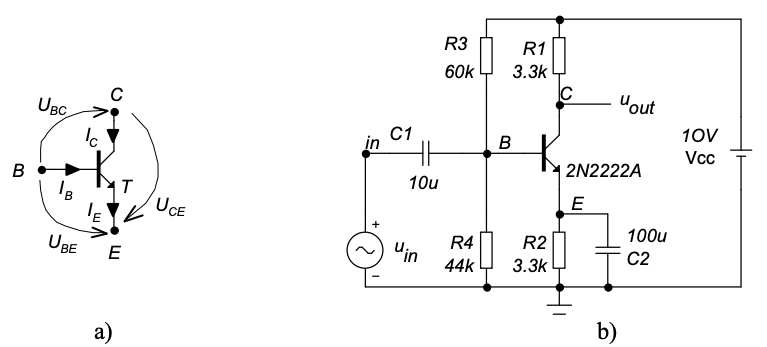
\includegraphics[width=\textwidth]{pracovni_bod_tranzistoru.png}
    \caption{\label{pracovni_bod_tranzistoru}}
\end{figure}

Pokud tranzistory zapojíme do zapojení na \obr{pracovni_bod_tranzistoru} b) při \(U_{in} = 0\) ustálí se jeho veličiny na konkrétním bodě, tento bod označujeme \(Q\) a nazýváme ho stejnosměrný pracovní bod tranzistoru.
Aby mohl tranzistor fungovat jako zesilovač správně je nutné aby nastavení pracovního bodu umožňovalo v oběma směry dostatečný rozkmit výstupního signálu v dostatečné míře bez přílišného zkreslení.
Pracovní bod se proto obvykle nastavuje tak aby v ustáleném stavu platilo \(U_{out} = \frac{1}{2}V_{cc}\)

\vspace{1mm}
\begin{wrapfigure}{r}{0.5\textwidth}
  % \centering
  \vspace{-10mm}
  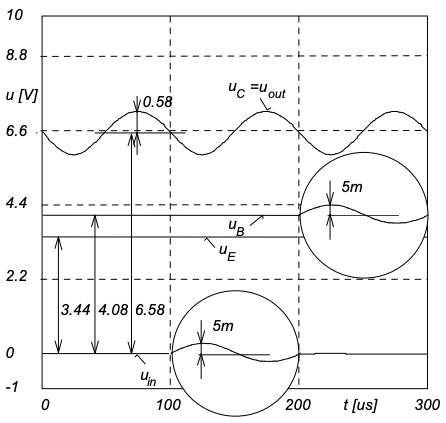
\includegraphics[width=0.5\textwidth]{vstup-baze-vystup.png}
  \caption{\label{vstup_baze_vystup}}
\end{wrapfigure}
Abychom mohli na tento zesilovač přivést signál s jiným středním napětím neš jaké je na bázi tranzistoru, přípojíme vstup zesilovače na bázi skrz kapacitu \(C_1\).
Tato kapacita musí být dostatečně velká aby se pro signál o požadované frekvenci dala považovat za zkrat.
Na \obr{vstup_baze_vystup} je zobrazen možný procházející signál.

Při nastavování pracovního bodu je mimo jiné nezbytné znát následující vztahy
\begin{equation}
    I_C=I_B\cdot\beta \quad \quad I_{E}=I_{B}+I_{C}
    \label{proud_kolektoru}
\end{equation}
\newpage

\section{Počítačové cvičení}
\begin{figure}[H]
  \begin{minipage}[t]{0.5\textwidth}
    \subsection{Bipolární tranzistor}
  \end{minipage}
  \begin{minipage}[t]{0.5\textwidth}
    \vspace{-15mm}
    \begin{figure}[H]
      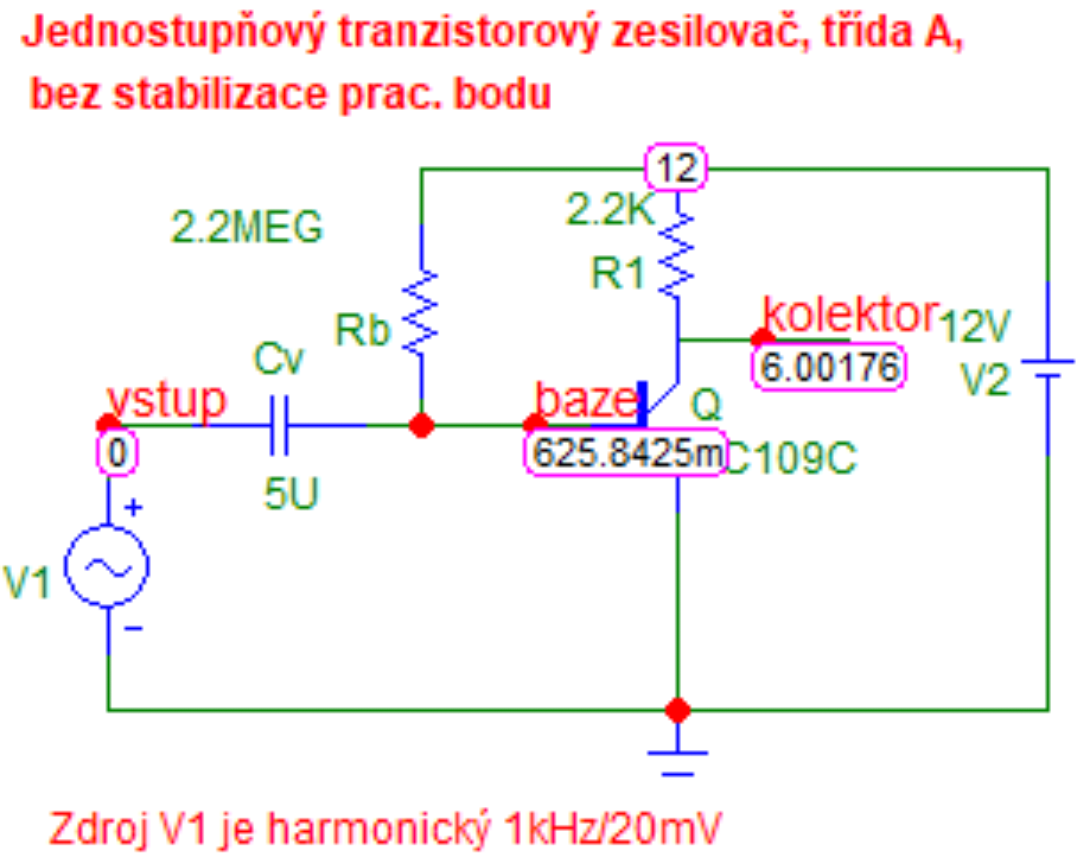
\includegraphics[width=\textwidth]{PC/BJT/prac_bod.png}
      % \addlegendentry{test}
      \caption{\label{prac_bod} Stejnosměrné nastavení pracovního bodu}
    \end{figure}
  \end{minipage}
  
  \begin{minipage}[t]{0.33\textwidth}
    \begin{figure}[H]
      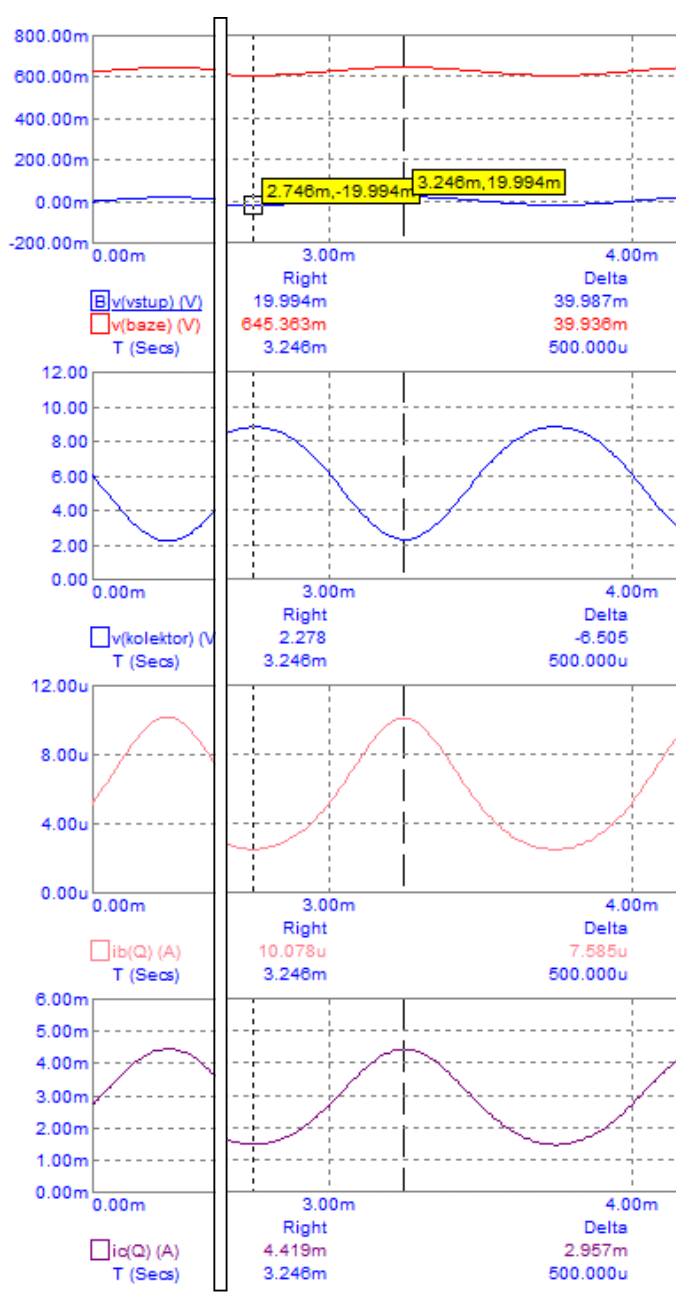
\includegraphics[width=\textwidth]{PC/BJT/sim_1.png}
      % \addlegendentry{test}
      \caption{\label{sim_1} Odezva na základní sinusoví signál}
    \end{figure}
  \end{minipage}
  \hfill
  \begin{minipage}[t]{0.25\textwidth}
    \begin{figure}[H]
      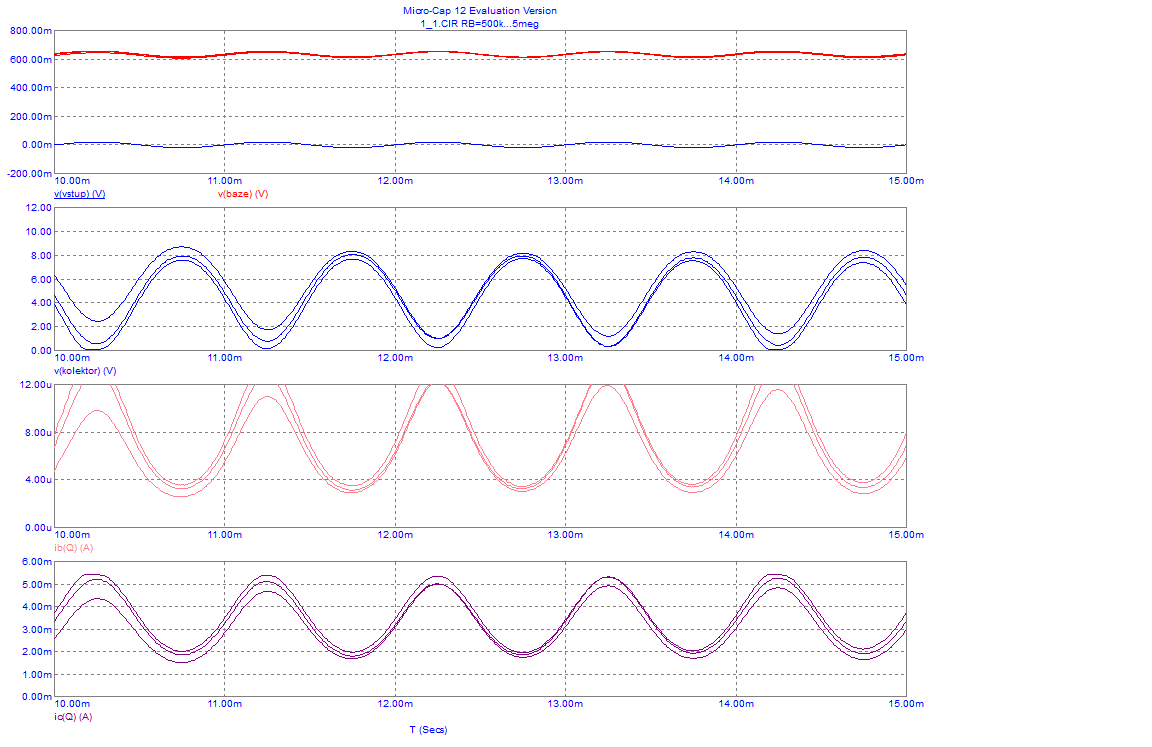
\includegraphics[width=\textwidth]{PC/BJT/Tranzient_analyza_4.png}
      \caption{\label{Tranzient_analyz_4} Sinusový průběh při změně \(R_b\)}
    \end{figure}
  \end{minipage}
  \hfill
  \begin{minipage}[t]{0.3\textwidth}
    \begin{figure}[H]
      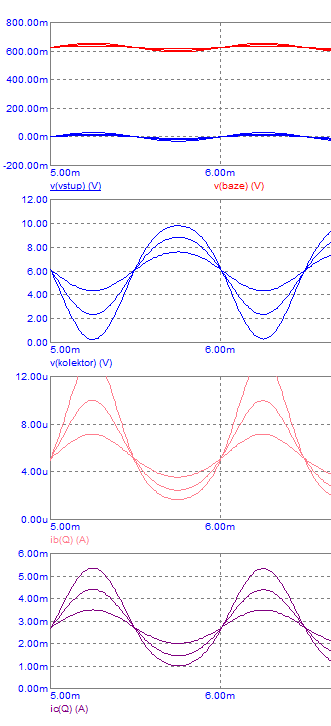
\includegraphics[width=\textwidth]{PC/BJT/Tranzient_analyza_3.png}
      \caption{\label{Tranzient_analyz_5 } Sinusový průběh při změně \(U_{in}\)}
    \end{figure}
  \end{minipage}
\end{figure}

\hfill
\begin{figure}[H]
  \includegraphics[width=\textwidth]{PC/BJT/Sirka_pasma.png}
  \caption{\label{sirka_pasma} Šířka pásma při \(C_v = 5\-[\mu F]\)}
\end{figure}
\begin{figure}[H]
  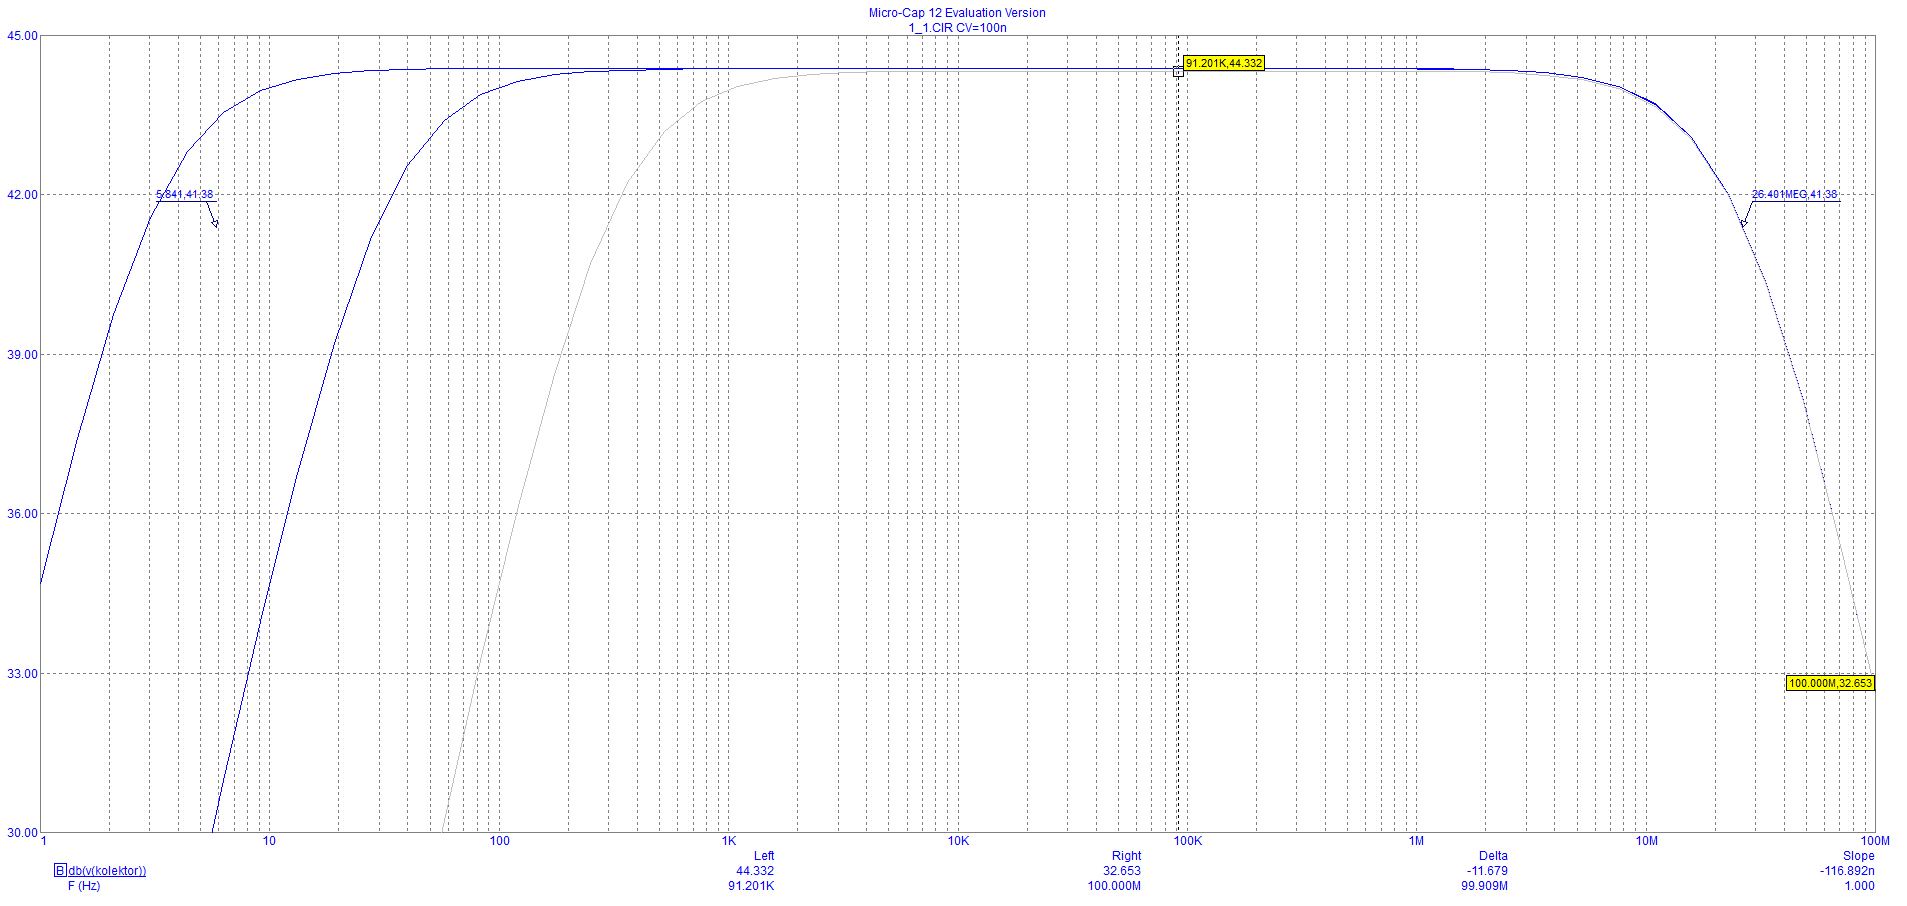
\includegraphics[width=\textwidth]{PC/BJT/Step_sirka_pasma.png}
  \caption{\label{Pohyb_sirky_pasma} Šířka pásma při změně \(C_v = 0.1;1;10\-[\mu F]\)}
\end{figure}
Je vidět že zmenšení kapacitoru znamená omezení šířky pásma v dolní části, nikoliv v horní.

\newpage

\begin{figure}[H]
  \begin{minipage}[t]{0.4\textwidth}
    \subsection{Unipolární tranzistor}
  \end{minipage}
  \begin{minipage}[t]{0.6\textwidth}
    \begin{figure}[H]
      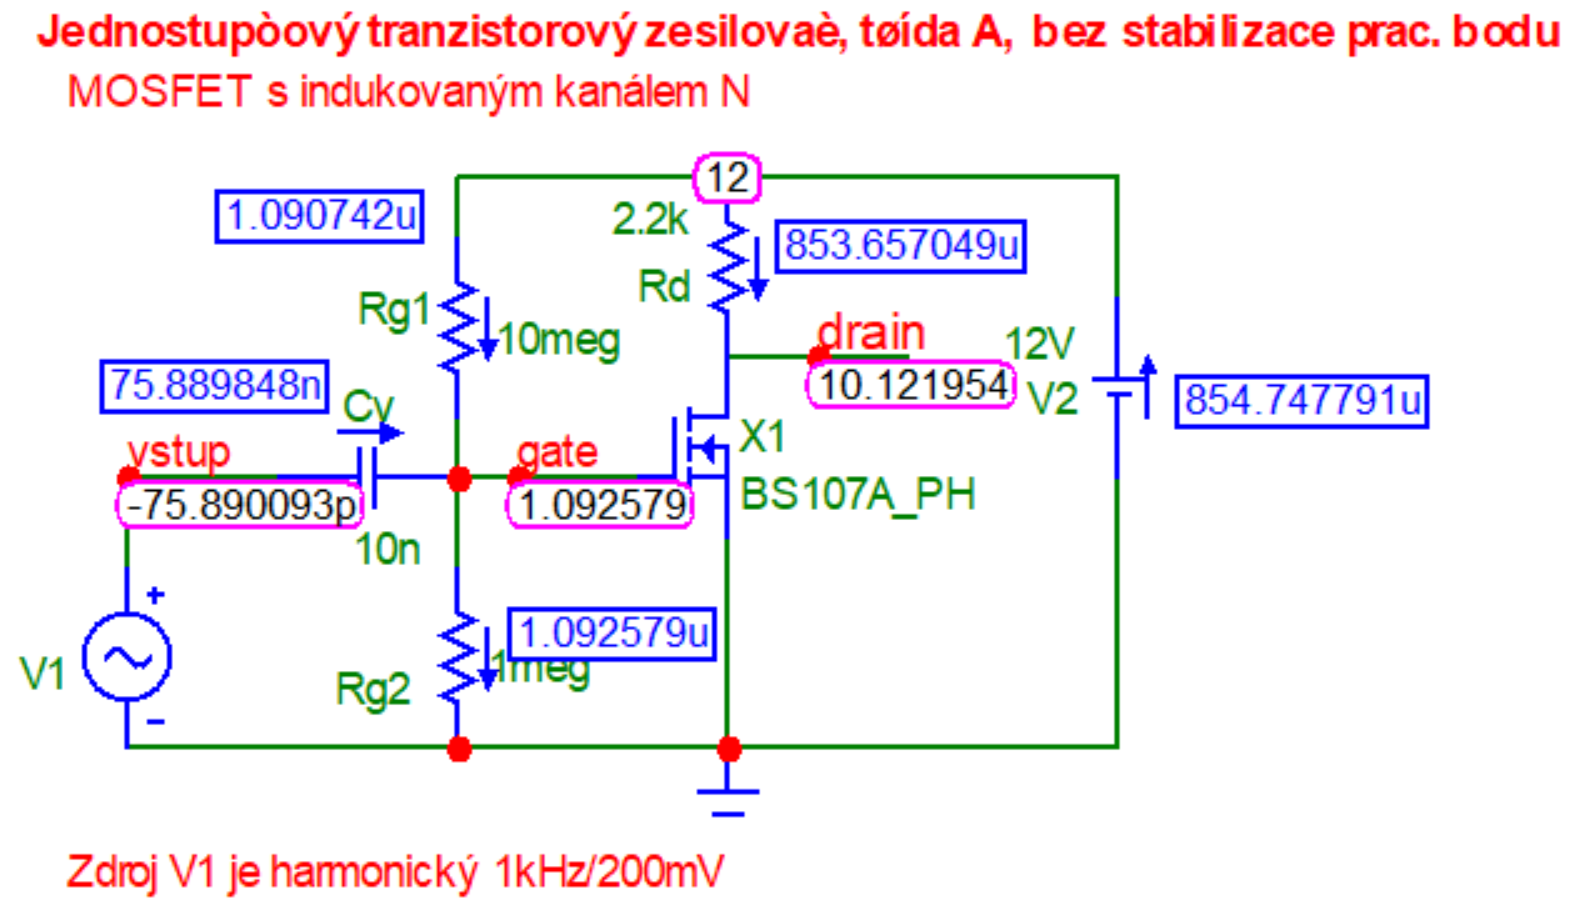
\includegraphics[width=\textwidth]{PC/UNI/napeti_a_proudy.png}
      \caption{\label{UNI_naperi_a_proudy} Stejnosměrné nastavení pracovního bodu}
    \end{figure}
  \end{minipage}
  
  \begin{minipage}[t]{0.30\textwidth}
    \begin{figure}[H]
      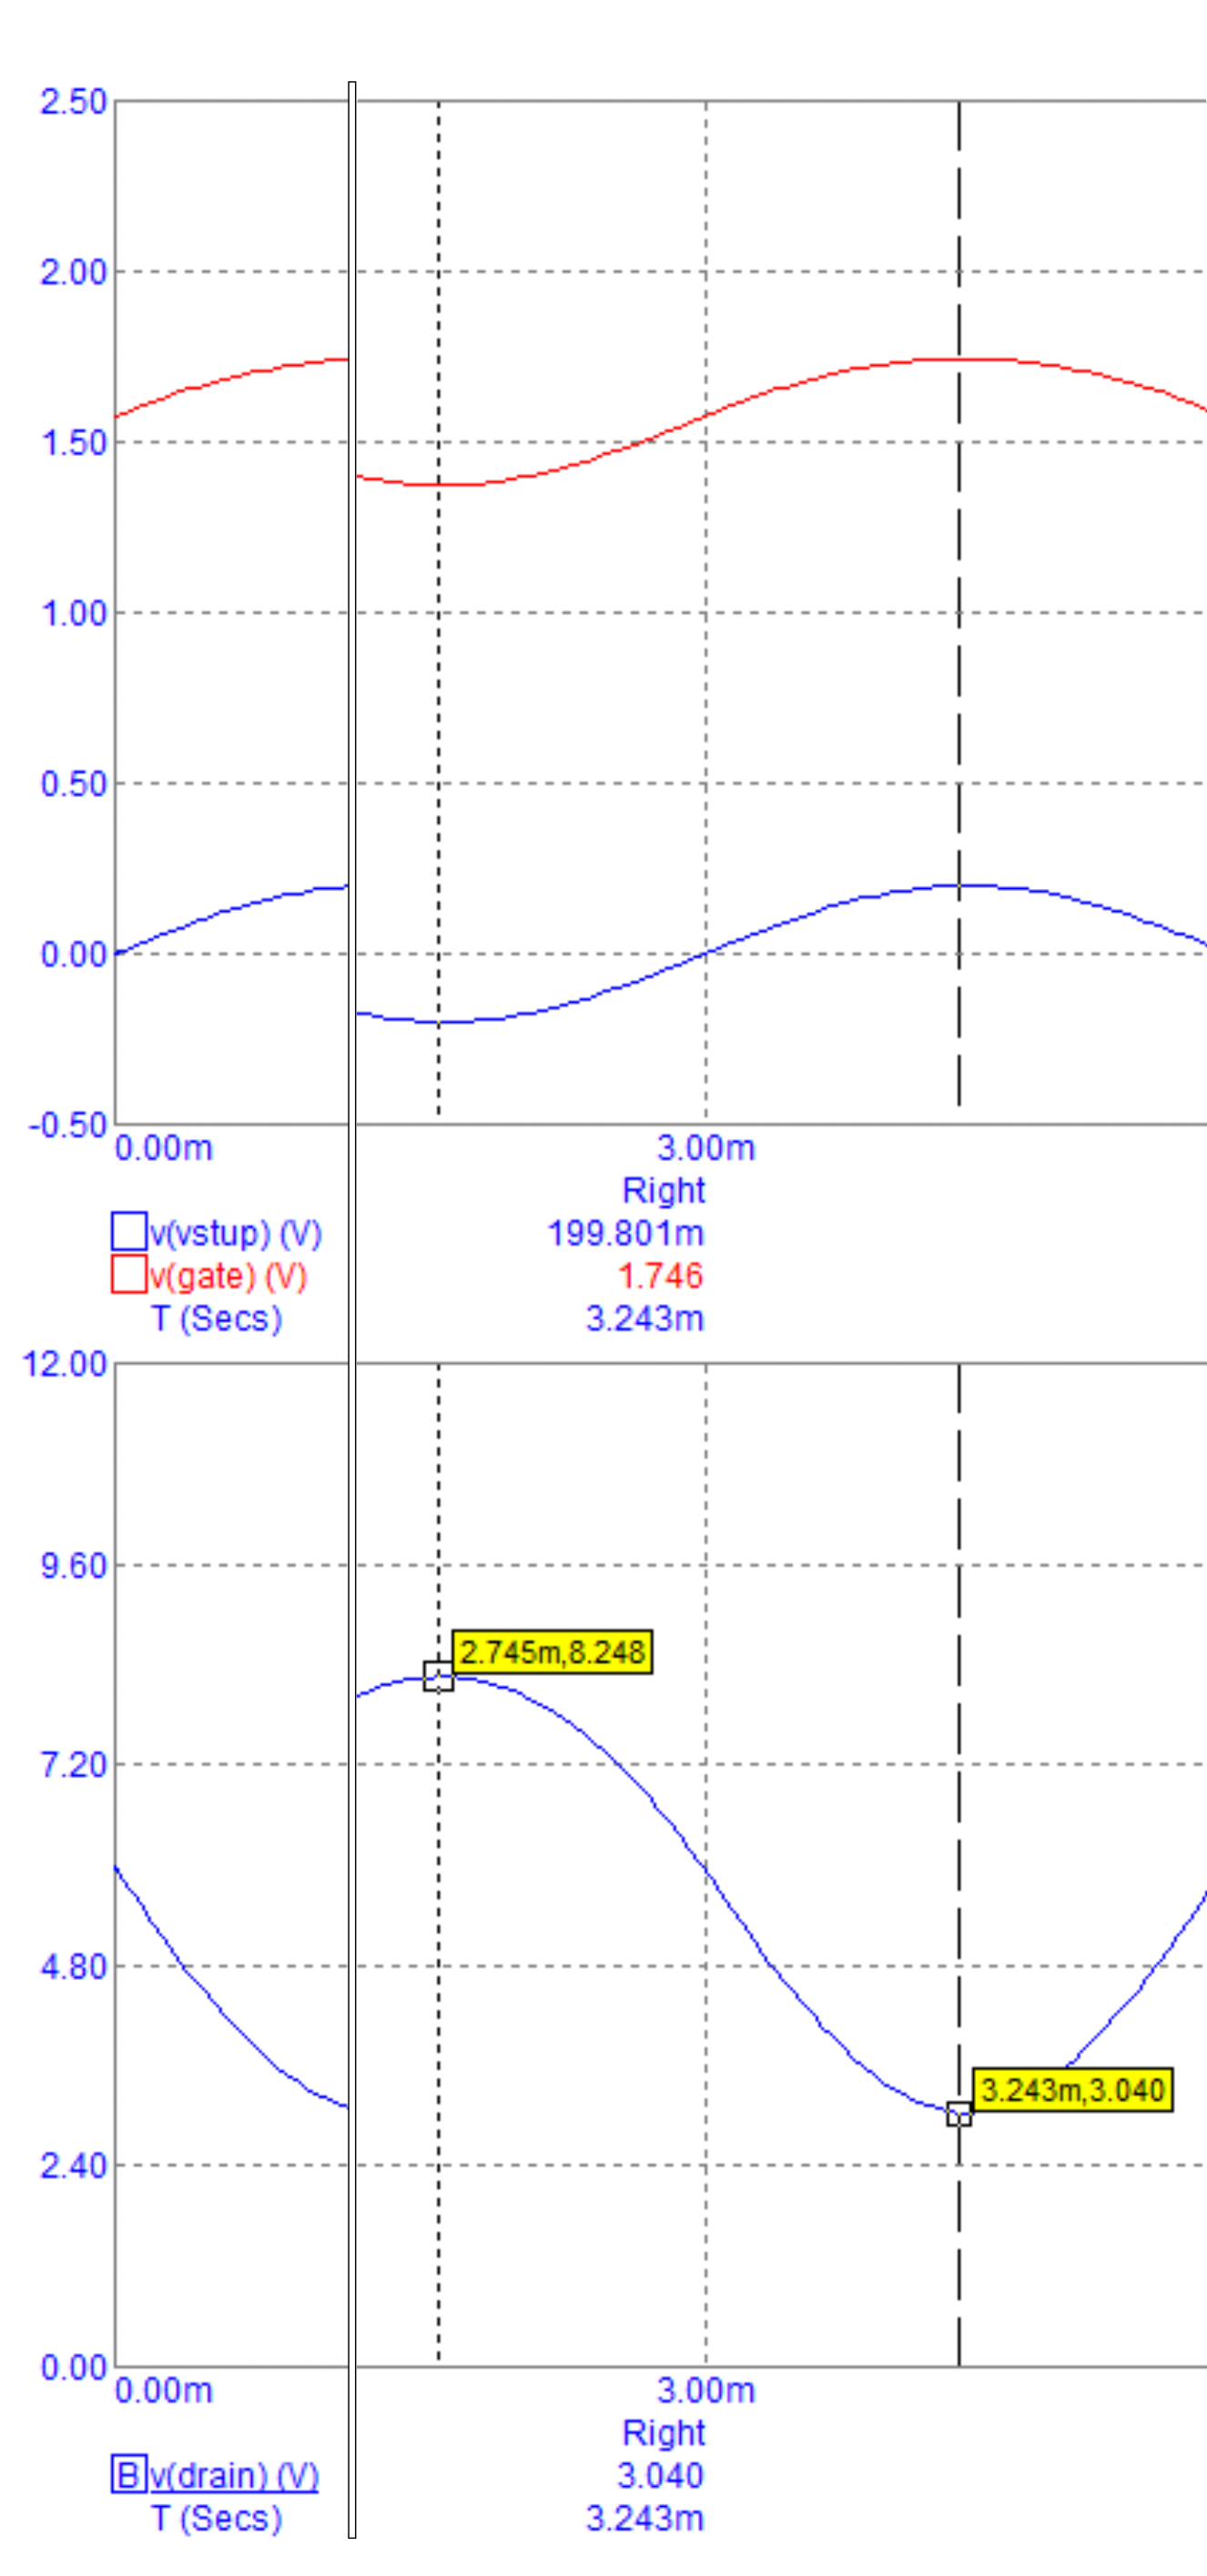
\includegraphics[width=\textwidth]{PC/UNI/UNI_Tranzient_1_3_redukovano.png}
      \caption{\label{UNI_Tranzient_reduk_1} Odezva na základní sinusoví signál}
    \end{figure}
  \end{minipage}
  \hfill
  \begin{minipage}[t]{0.33\textwidth}
    \begin{figure}[H]
      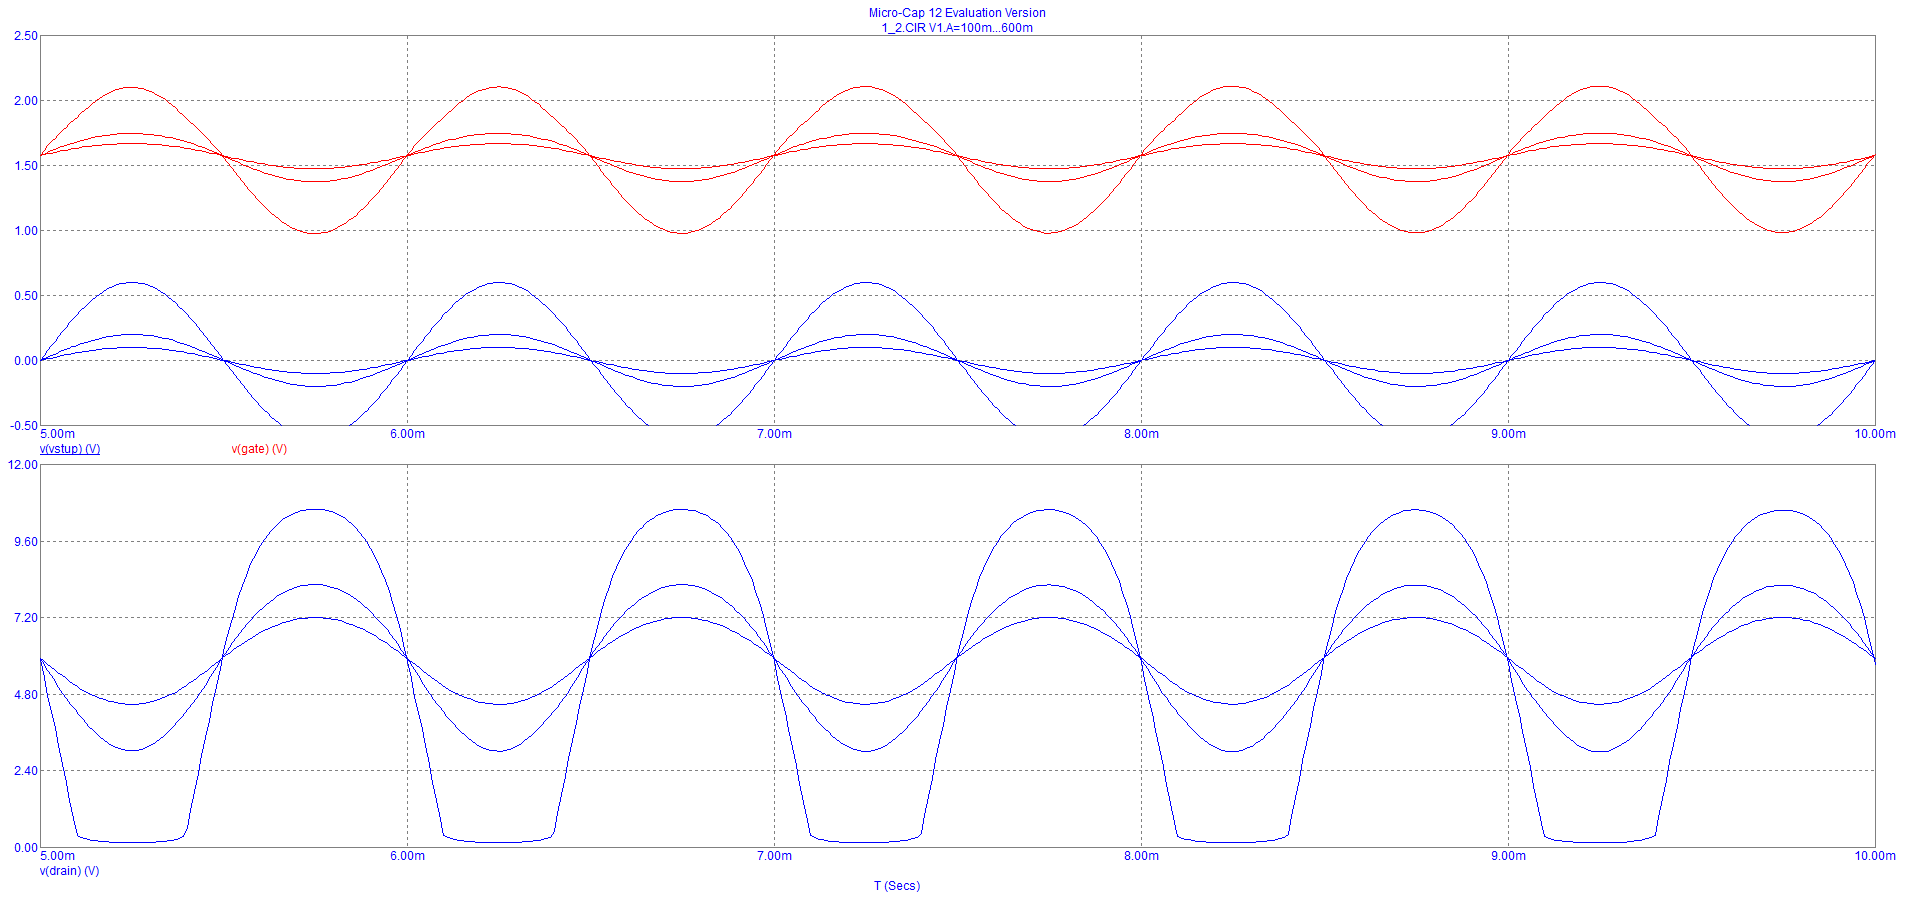
\includegraphics[width=\textwidth]{PC/UNI/UNI_Tranzient_2_1.png}
      \caption{\label{NUI_Tranzient_2} Sinusový průběh při změně \(R_b\)}
    \end{figure}
  \end{minipage}
  \hfill
  \begin{minipage}[t]{0.35\textwidth}
    \begin{figure}[H]
      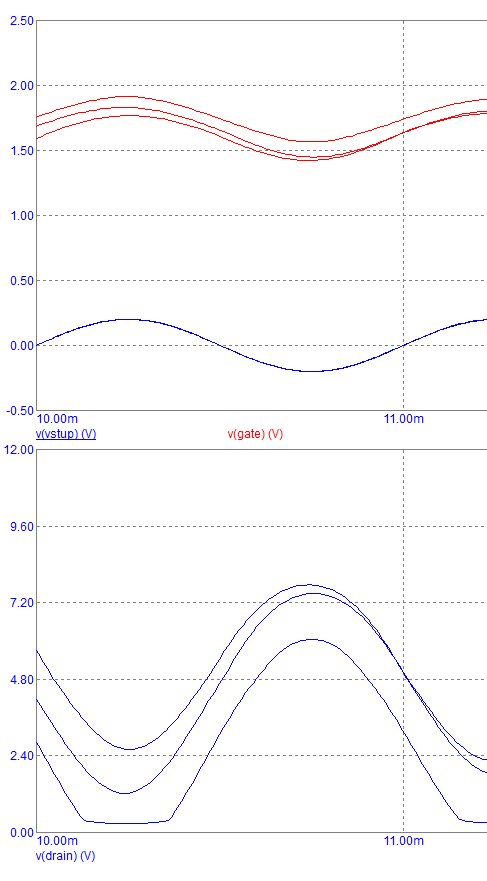
\includegraphics[width=\textwidth]{PC/UNI/posun_prac_podu.png}
      \caption{\label{Posun_prac_bodu} Sinusový průběh při změně \(U_{in}\)}
    \end{figure}
  \end{minipage}
\end{figure}

\begin{figure}[H]
	% \begin{minipage}[t]{0.45\textwidth}
  %   \vspace{-5mm}
  %   \begin{figure}[H]
  %     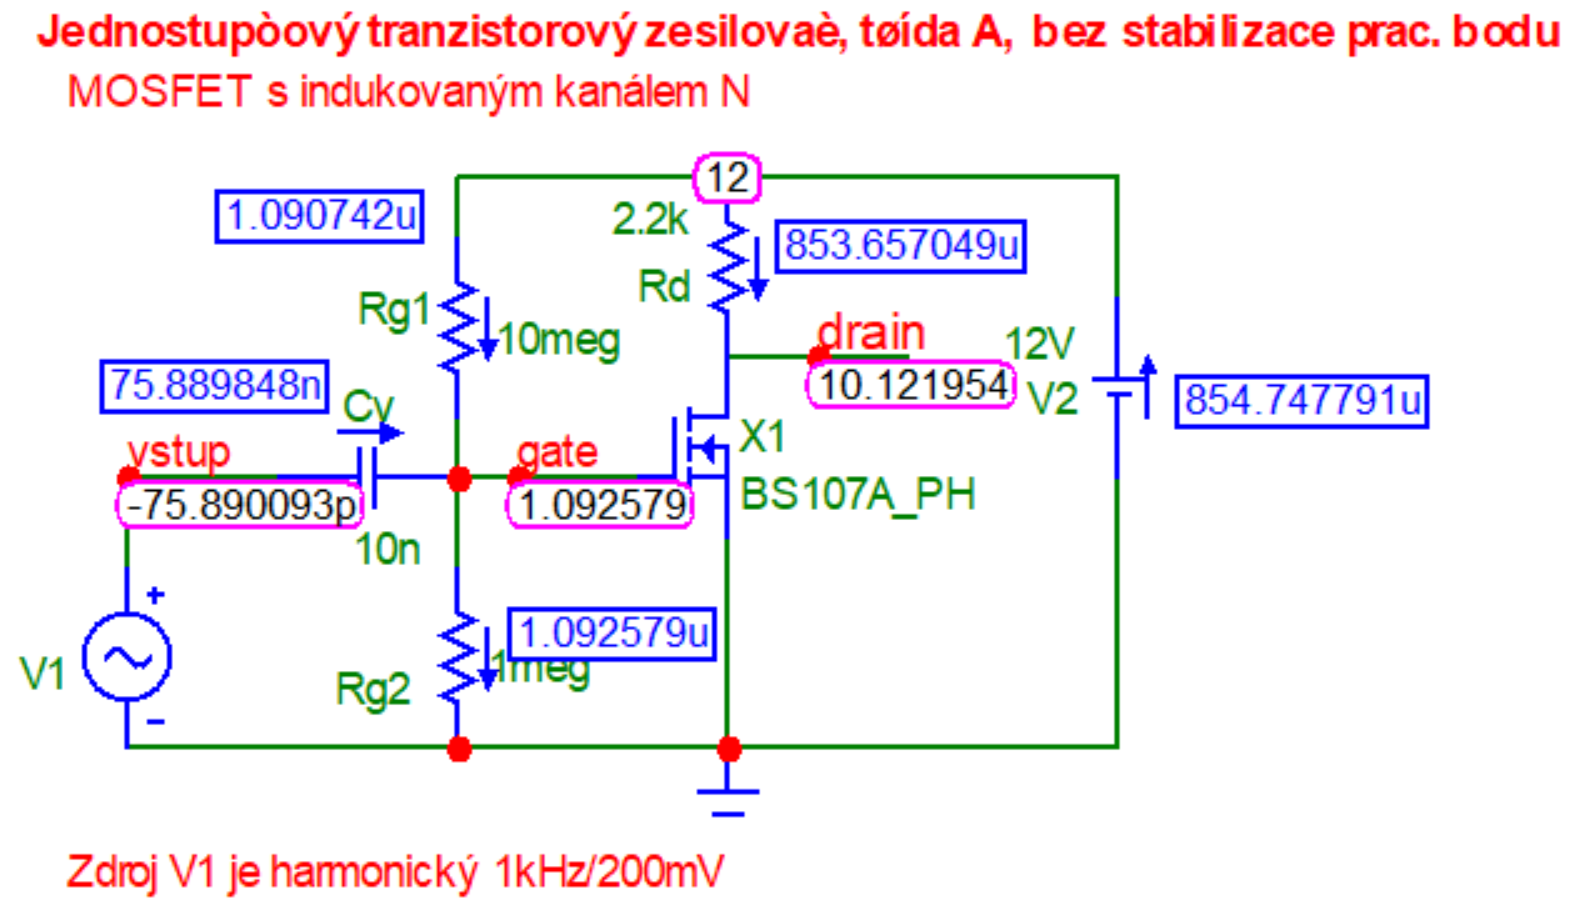
\includegraphics[width=\textwidth]{PC/UNI/napeti_a_proudy.png}
  %     % \addlegendentry{test}
  %     \caption{\label{prac_bod_sim_1} Stejnosměrné nastavení pracovního bodu}
  %   \end{figure}
  % \end{minipage}
  \hfill
  \begin{minipage}[t]{0.45\textwidth}
    \vspace{-10mm}
    \begin{figure}[H]
      % \addlegendentry{test}
      \caption{\label{prac_bod_sim_1} Odezva na základní sinusoví signál}
    \end{figure}
  \end{minipage}
\end{figure}


\begin{figure}[H]
	\begin{minipage}[t]{1\textwidth}
    \begin{figure}[H]
      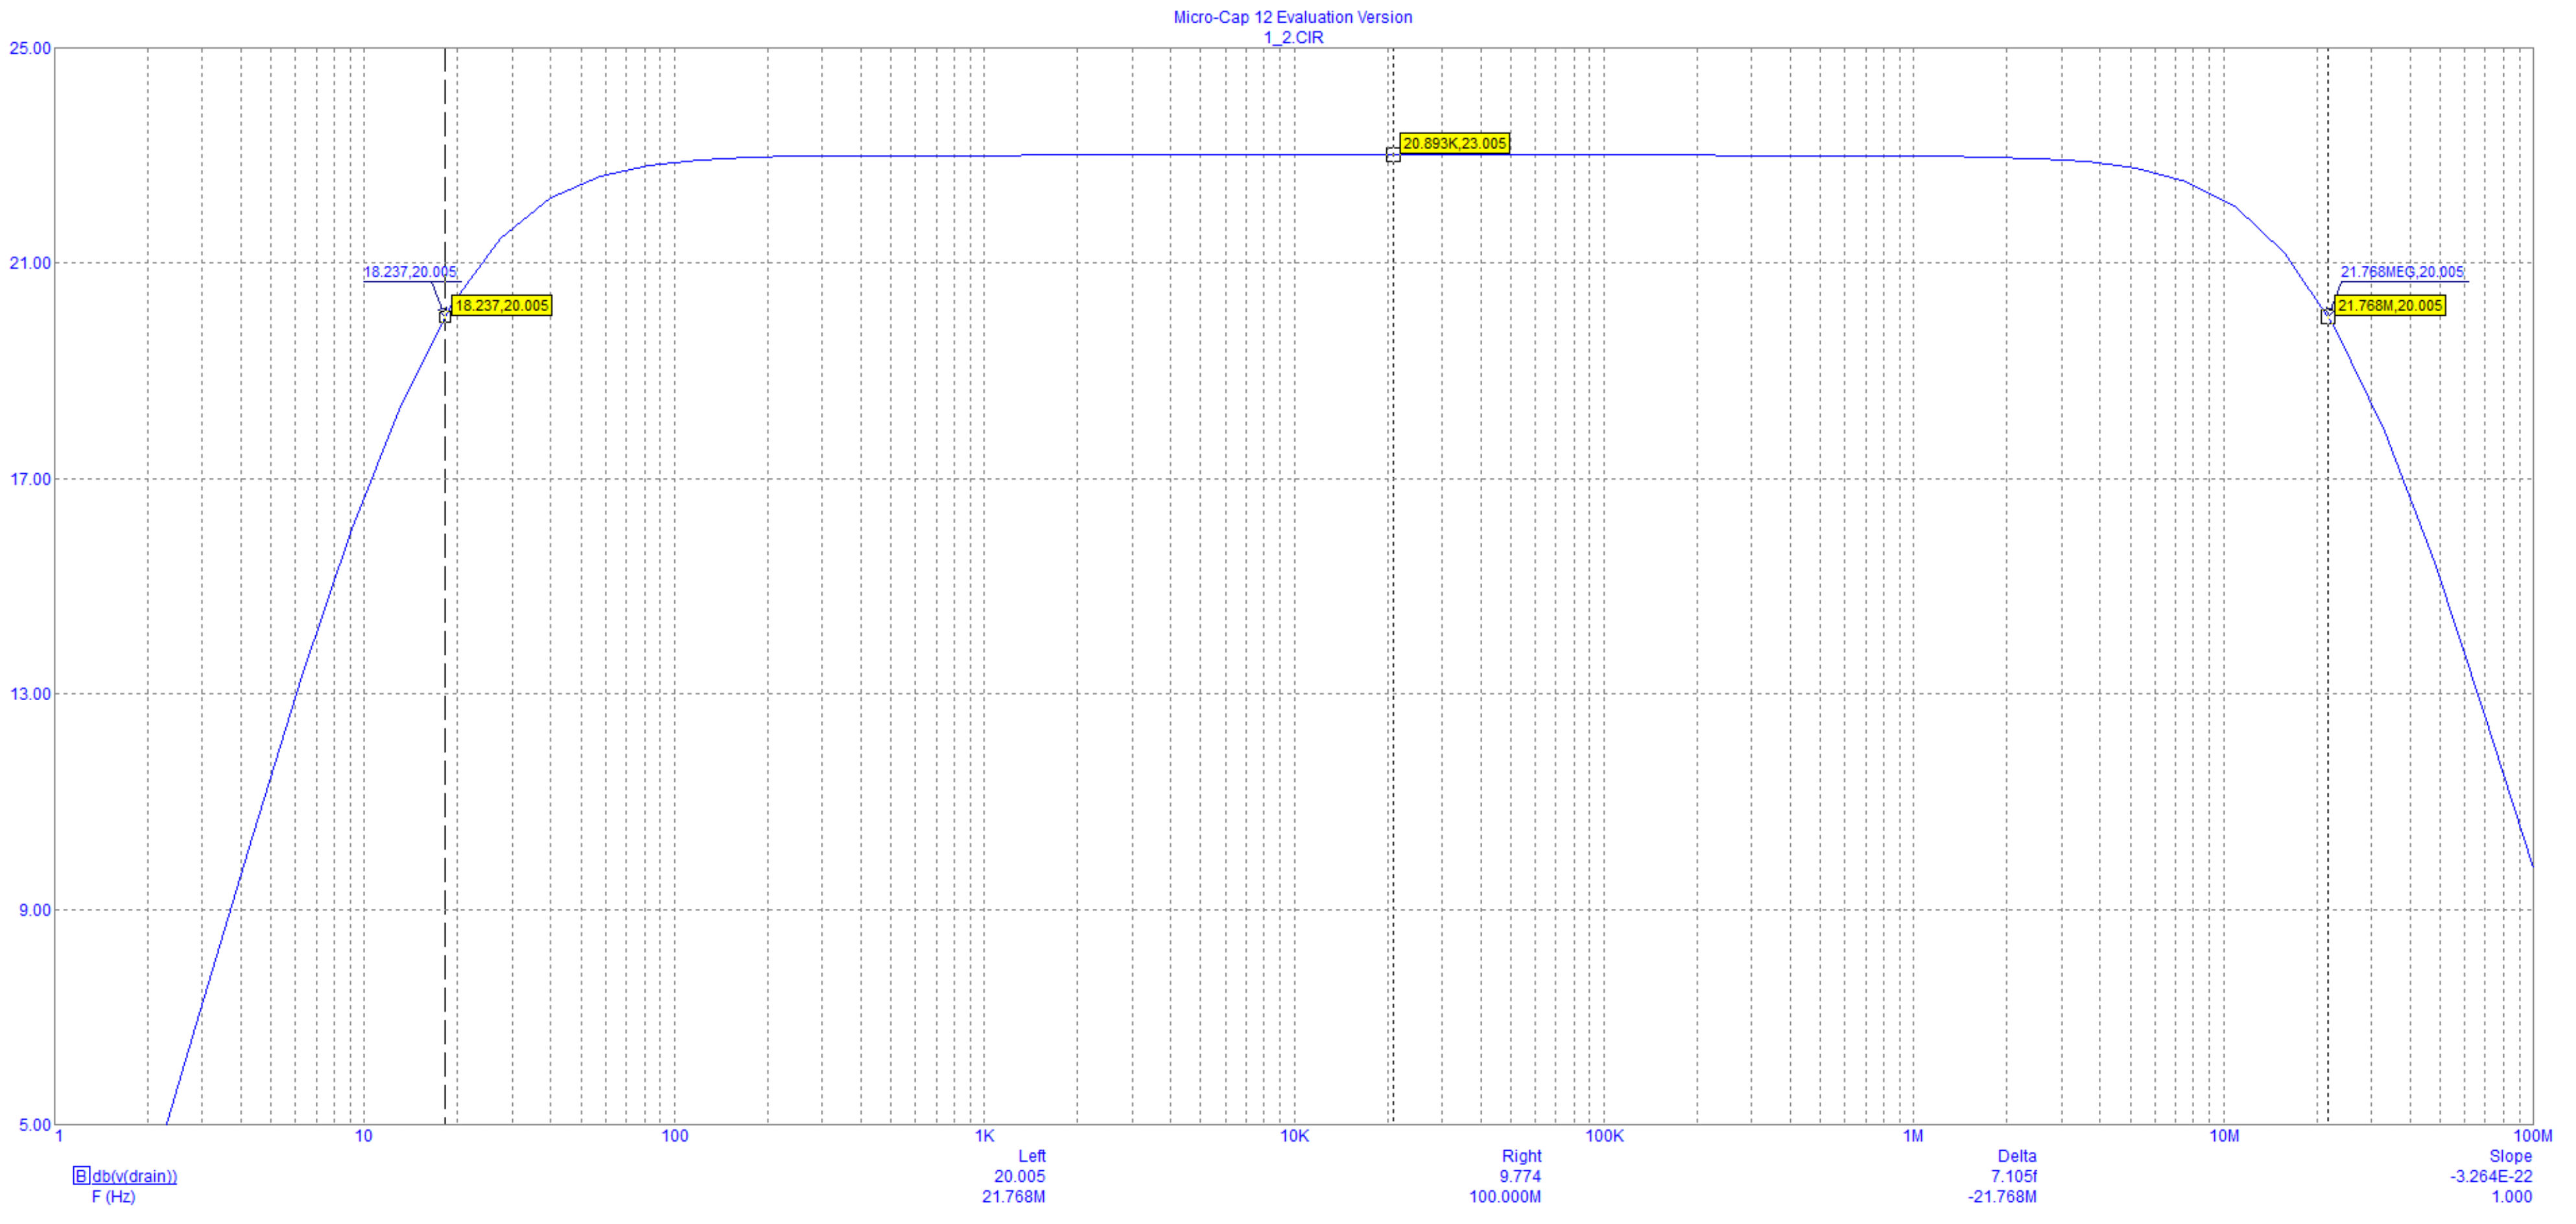
\includegraphics[width=\textwidth]{PC/UNI/UNI_sirka_pasma_2.png}
      \caption{\label{sirka_pasma} Šířka pásma při \(C_v = 5\-[\mu F]\)}
    \end{figure}
    \begin{figure}[H]
      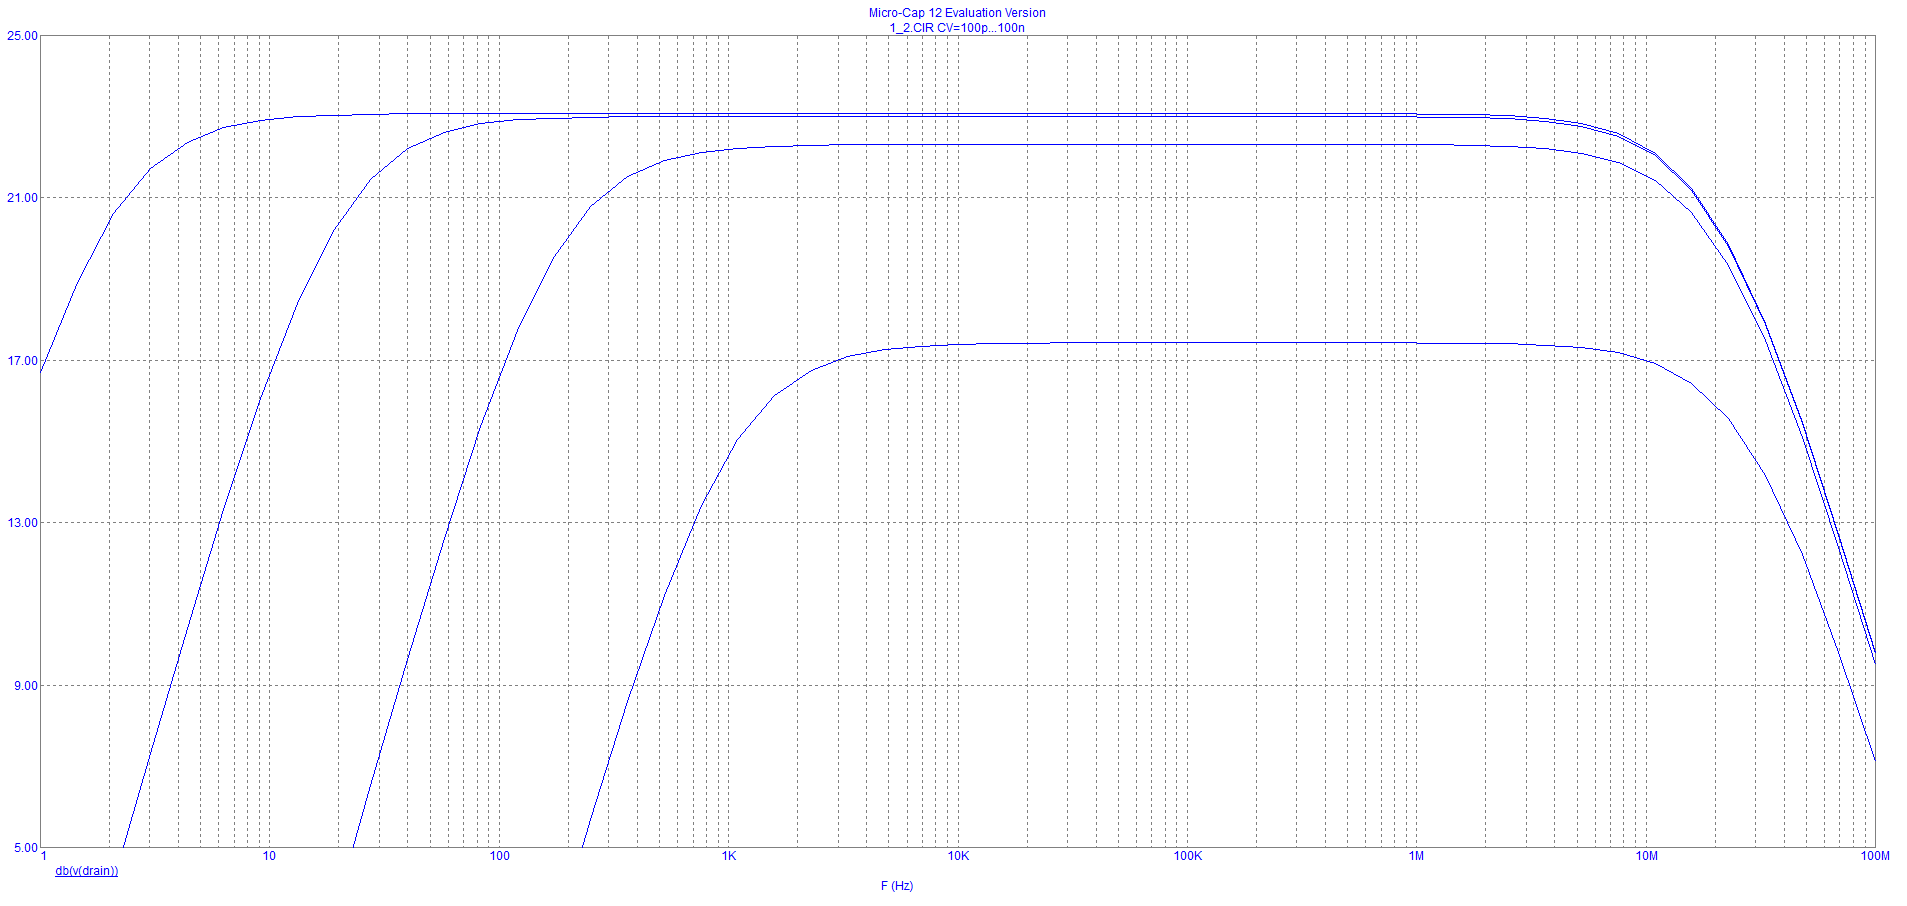
\includegraphics[width=\textwidth]{PC/UNI/UNI_sirky_pasma.png}
      \caption{\label{Pohyb_sirky_pasma} Šířka pásma při změně \(C_v = 0.1;1;10\-[\mu F]\)}
    \end{figure}
  \end{minipage}
  \begin{minipage}[t]{1\textwidth}
    Je vidět že zmenšení kapacitoru znamená omezení šířky pásma v dolní části, nikoliv v horní.
    Na rozdíl od bipolárního tranzistoru, kde se zmenšuje šířka pásma ale maximální zesílení zůstává stejné, v tomto zapojení zvýšení kapacity znamená zároveň zvýšení maximálního zesílení.
  \end{minipage}
\end{figure}

\newpage
\section{Laboratorní cvičení}
% \subsections{zadání}
% Nejprve sestavte obvod bez vazebního kondenzátoru a zdroje signálu. Změnou odporu Rb
% nastavte ss napětí na kolektoru tranzistoru 6 V. Změřte všechna uzlová napětí a z nich dopočtěte
% větvové proudy. Porovnejte s výsledky z NC a PC.
% Doplňte obvod o Cv a generátor signálu. Proveďte „oživení“ zesilovače pomocí osciloskopu.
% Zesilovač nesmíte přebudit výstupní napětí nesmí vykazovat zkreslení. Měřte při kmitočtu
% 1 kHz. Zakreslete časové průběhy vstupního napětí, napětí na bázi a na kolektoru, včetně ss
% posunutí. Změřte amplitudy a vypočtěte z nich střídavá zesílení.

\begin{figure}[H]
	\begin{minipage}[t]{0.6\textwidth}
    Měřili jsme s tranzistorem BC55 u kterého jsme na začátku naměřili \(\beta = 422\)
    Nejprve jsme sestavili obvod a pomocí potenciometru jsme nastavili pracovní bod dle \tab{tab_pracovni_bod}.
    % \vspace{-5mm}
    \begin{table}[H]
      % \centering
      \begin{tabular}{|c|c|c|c|c||c|c|} 
        \hline
         \(U_{cc}\-[V]\) & \(U_{C}\-[V]\)  & \(R_b\-[M\Omega]\) &	\(R_c\-[K\Omega]\) & \(U_{b}\-[V]\) & \(I_{C}\-[mA]\) & \(I_{b}\-[\mu A]\)  \\ \hline
         12              & 6.1             & 2.5                & 2.2                & 0.61           & 2.68            & 6.36                \\ \hline
      \end{tabular}
      \caption{\label{tab_pracovni_bod} Nastavení obvodu}
    \end{table}
   	\(\bullet\) kanál 1 ... \(U_{in}\)  \qquad 	\(\bullet\) kanál 2 ... \(U_{out}\)
  \end{minipage}
  \hfill
	\begin{minipage}[t]{0.4\textwidth}
    \begin{figure}[H]
      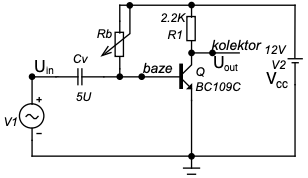
\includegraphics[width=\textwidth]{obvod-z-laborky.png}
      \caption{\label{obvod_z_laborky}}
    \end{figure}
  \end{minipage}
\end{figure}


\begin{figure}[H]
	\begin{minipage}[t]{0.6\textwidth}
    \vspace{-20mm}
    \begin{figure}[H]
      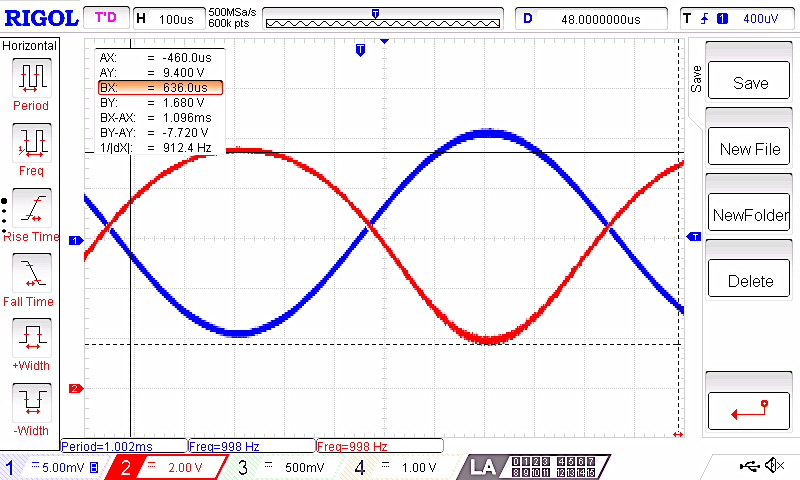
\includegraphics[width=\textwidth]{LAB/NewFile2.png}
      \caption{\label{obvod_z_laborky}}
    \end{figure}
  \end{minipage}
  \hfill
	\begin{minipage}[t]{0.35\textwidth}
    Dále jsme na  vstup přivedly signál o napětí \(U_{in} = 1\-[V]\) a frekvenci \(f = 1\-[kHz]\). 
    Díky hodnotě vstupního napětí rovnou vidíme zesílení tohoto zapojení \(A = 7.72\-[-]\).
  \end{minipage}
\end{figure}

\begin{figure}[H]
	\begin{minipage}[t]{0.6\textwidth}
    \vspace{-10mm}
    \begin{figure}[H]
      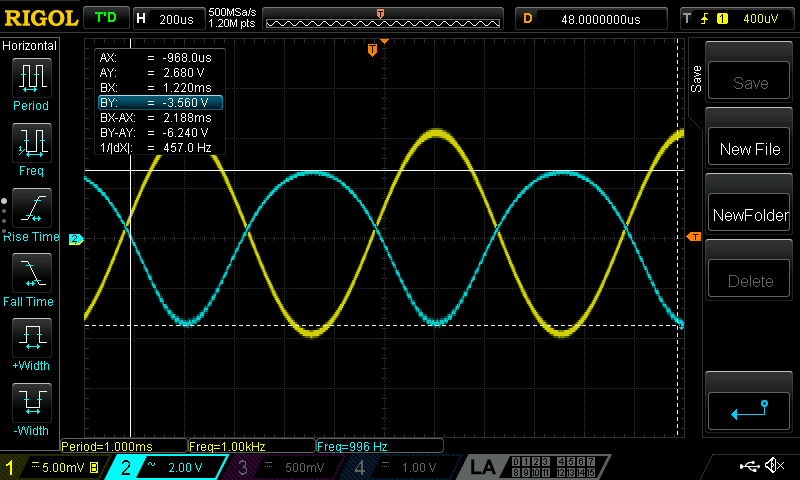
\includegraphics[width=\textwidth]{LAB/NewFile4.png}
      \caption{\label{obvod_z_laborky}}
    \end{figure}
  \end{minipage}
  \hfill
	\begin{minipage}[t]{0.35\textwidth}
    Dále jsme přenastavili pracovní bod dle tabulky:
    \begin{table}[H]
      % \centering
      \hspace{-5mm}
      \small
      \begin{tabular}{|c|c|c|c|c|} 
        \hline
        \(U_{cc}\-[V]\) & \(U_{C}\-[V]\)  & \(R_b\-[M\Omega]\) & \(R_c\-[K\Omega]\) & \(U_{b}\-[V]\)  \\ \hline
        12              & 7.6             & 3.44               & 2.2                & 0.61            \\ \hline
        \hline
        \(I_{C}\-[mA]\) & \(I_{b}\-[\mu A]\) & - & - & - \\\hline
        2.00            & 4.74               & - & - & - \\\hline
      \end{tabular}
      \normalsize
      \caption{\label{tab_pracovni_bod_rozladeni1} Přenastavení obvodu 1}
    \end{table}
  \end{minipage}
\end{figure}

\begin{figure}[H]
	\begin{minipage}[t]{0.6\textwidth}
    \vspace{-10mm}
    \begin{figure}[H]
      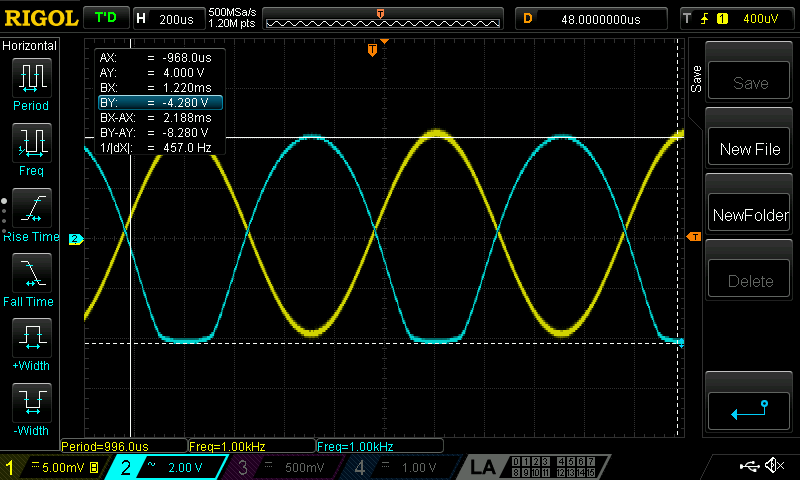
\includegraphics[width=\textwidth]{LAB/NewFile6.png}
      \caption{\label{obvod_z_laborky}}
    \end{figure}
  \end{minipage}
  \hfill
	\begin{minipage}[t]{0.35\textwidth}
    Dále jsme přenastavili pracovní bod dle tabulky:
    \begin{table}[H]
      % \centering
      \hspace{-5mm}
      \small
      \begin{tabular}{|c|c|c|c|c|} 
        \hline
        \(U_{cc}\-[V]\) & \(U_{C}\-[V]\)  & \(R_b\-[M\Omega]\) & \(R_c\-[K\Omega]\) & \(U_{b}\-[V]\)  \\ \hline
        12              & 4.5             & 1.90               & 2.2                & 0.61            \\ \hline
        \hline
        \(I_{C}\-[mA]\) & \(I_{b}\-[\mu A]\) & - & - & - \\\hline
        3.41            & 8.08               & - & - & - \\\hline
      \end{tabular}
      \normalsize
      \caption{\label{tab_pracovni_bod_rozladeni1} Přenastavení obvodu 1}
    \end{table}
  \end{minipage}
\end{figure}


\end{document}
